\documentclass[a4paper,12pt]{article}
\usepackage[a4paper,top=1.3cm,bottom=2cm,left=1.5cm,right=1.5cm,marginparwidth=0.75cm]{geometry}
%%% Работа с русским языком
\usepackage{cmap}					% поиск в PDF
\usepackage{mathtext} 				% русские буквы в фомулах
\usepackage[T2A]{fontenc}			% кодировка
\usepackage[utf8]{inputenc}			% кодировка исходного текста
\usepackage[english,russian]{babel}	% локализация и переносы

\usepackage{graphicx}
\usepackage{mathtools}
\usepackage{wrapfig}
\usepackage{tabularx}
\usepackage{amssymb}
\usepackage{hyperref}
\usepackage[rgb]{xcolor}
\hypersetup{colorlinks=true,urlcolor=blue}
\setcounter{secnumdepth}{0}
%% Шрифты
\usepackage{euscript}	 % Шрифт Евклид
\usepackage{amsmath}
\usepackage{mathtools}
%%% Заголовок
\author{Tsvetkova Amelia}
\title{Лабораторная работа по общей физике}

\date{\today}
\begin{document}
\begin{titlepage}
    \newpage
    \begin{center}
    {\large МОСКОВСКИЙ ФИЗИКО-ТЕХНИЧЕСКИЙ ИНСТИТУТ (НАЦИОНАЛЬНЫЙ ИССЛЕДОВАТЕЛЬСКИЙ УНИВЕРСИТЕТ)}
    \vspace{1cm}

    {\largeФизтех-школа аэрокосмических технологий}
    \vspace{6em}
    \end{center}
    
    \vspace{1.2em}

    \begin{center}
    \Large Лабораторная работа №4.3.2 \\
    Дифракция света на ультразвуковой волне в жидкости
    \linebreak
    \end{center}
    
    \vspace{11em}
    
    \begin{flushright}
                       {\large Работу выполнила\\
                       Цветкова Амелия Антоновна\\
                       Б03-303 }
    \end{flushright}

    \vspace{\fill}

    \begin{center}
    Долгопрудный, 2025
    \end{center}

    \end{titlepage}

\paragraph{Цель работы:} изучение дифракции света на синусоидальной акустической решетке и наблюдение фазовой решетки методом темного поля.

\paragraph{В работе используются:} оптическая скамья, осветитель, два длиннофокусных объектива, кювета с жидкостью, кварцевый излучатель с микрометрическим винтом, генератор ультразвуковой частоты, линза, вертикальная нить на рейтере, микроскоп.

\section{Теоретические сведения}

\subsection{Примеры расчета дифракции спектральным методом}

\subsubsection{Дифракция Френеля на амплитудной синусоидальной решетке}
Функция пропускания решетки с периодом $d=2\pi/\Omega$:
$$
t(x) = 1+m\cos{\Omega x} \quad (m < 1)
$$

Пусть решетка освещается плоской нормально падающей волной амплитуды $a$, т.е. $f_s(x)=ae^{ikz}$. Решетка установлена в плоскости $z=0$, поэтому $f_z=a$. Тогда $f_0(x) = a(1+m\cos{\Omega x})$. С помощью $\cos{\Omega x}=\frac{1}{2}e^{i\Omega x} + \frac{1}{2}e^{-i\Omega x}$ находим
$$
f_0(x) = a+\frac{am}{2}e^{i\Omega x} + \frac{am}{2}e^{-i\Omega x}
$$

Комплексная амплитуда волны в плоскости $z$ имеет вид:
$$
f(x,z)=ae^{ikz} + \frac{am}{2}e^{i(\Omega x + \sqrt{k^2-\Omega^2}z)} + \frac{am}{2}e^{i(-\Omega x+\sqrt{k^2-\Omega^2}z)}
$$
Первое слагаемое - волна с амплитудой $a$, бегущая вдоль оси $z$. Два других слагаемых - волны с амплитудами $\frac{am}{2}$ и пространственными частотами $\pm\Omega$. 

Полагаем, что период решетки $d = \frac{2\pi}{\Omega}$ существенно больше длины волны $\lambda$ и, значит, частота решетки много меньше $k$: $\Omega \ll k$. Тогда находим
$$
f(x,z)=ae^{ikz}+\frac{am}{2}e^{ikz} \cdot e^{i(\Omega x - \frac{z}{2k}\Omega^2)} + \frac{am}{2}e^{ikz}\cdot e^{i(-\Omega x-\frac{z}{2k}\Omega^2)}
$$
После преобразований получаем:
$$
f(x,z) = ae^{ikz}\Big[1+me^{-i\frac{z}{2k}\Omega^2}\cdot\cos{\Omega x}\Big]
$$

\subsubsection{Дифракция на фазовой синусоидальной решетке}
Функция пропускания $t(x)=e^{im\cos{\Omega x}}$. Будем полагать, что глубина модуляции фазы мала($m\ll 1$). Тогда
$$
t(x)\approx 1+im\cos{\Omega x}=1+\frac{im}{2}e^{i\Omega x} +\frac{im}{2}e^{-i\Omega x}
$$
Колебания, созданные наклонными волнами, отстают по фазе на $\pi/2$ от колебаний осевой волны.

\subsection{Визуализация фазовых объектов. Метод фазового контраста и метод темного поля}
Пусть фазовый объект - тонкая прозрачная пластинка, имеющаяа разный в разных точках показатель преломления, но не изменяющая амплитуду прошедшей волны. Функция пропускания такой пластинки $t(x)=e^{i\varphi(x)}$, где $\varphi(x)=kn(x)d$. При освещении пластинки плоской нормально падающей волной комплексная амплитуда волны есть $f_0(x)=e^{i\varphi(x)}$. 

Для визуализации фазового объекта установим в фурье-плоскости, на оптической оси, маленькую фильтрующую пластинку, которая, не изменяя амплитуды, вносит фазовую задержку $\pi/2$. В случае фазовой синусоидальной решетки с малой глубиной модуляции($m\ll 1$):
$$
f_0(x)=e^{im\cos{\Omega x}} \approx 1+im\cos{\Omega x} = 1 + \frac{im}{2}e^{i\Omega x} + \frac{im}{2}e^{-i\Omega x}
$$

Осевая плоская волна, фокусируясь линзой в начало координат фурье-плоскости($\xi=0$), проходит через фазовую фильтрующую пластинку, а две наклонные волны, фокусируясь в точки $\xi_{1,2}=\pm f\alpha =\pm f\frac{\Omega}{k}$, не "задевают" пластинку. Далее линза преобразует сферические волны, исходящие из этих точек, в плоские волны, которые, интерферируя, образуют изображение.

Поле в выходной плоскости:
$$
f(x)=e^{i\frac{\pi}{2}}+\frac{im}{2}e^{i\Omega x} + \frac{im}{2}e^{-i\Omega x}
$$
или
$$
f(x)=i\Big(1+\frac{m}{2}e^{i\Omega x} + \frac{m}{2}e^{-i\Omega x} \Big) = i(1 + m\cos{\Omega x})
$$

Таким образом, метод фазового контраста позволяет преобразовать исходную фазовую решетку в амплитудную решетку в плоскости изображения. Наблюдаемая картина интенсивности имеет вид:
$$
I(x)=|f(x)|^2 \approx (1+m\cos{\Omega x})^2 \approx 1 + 2m\cos{\Omega x}
$$

В методе темного поля вместо фазовой пластинки в $\pi/2$ в фурье-плоскости на оптической оси устанавливается непрозрачный маленький экран. Осевая плоская волна, фокусируясь линзой в начало  координат фурье-плоскости, поглощается непрозрачным экраном и не участвует в формировании изображения. Боковые же волны остаются без изменений. Поле в выходной плоскости имеет вид:
$$
f(x)=\frac{im}{2}e^{i\Omega x}+\frac{im}{2}e^{-i\Omega x}=im\cos{\Omega x}
$$
а картина интенсивности - $I(x)=m^2\cos^2{\Omega x}$

\subsection{Дифракция на ультразвуковой волне}
При прохождении ультразвуковой волны через жидкость в ней возникают периодические оптические неоднородности, обусловленные разницей значений коэффициента преломления.

Пусть УЗ-волна рааспространяется вдоль оси $X$ (рис. \ref{img1}) в жидкости, налитой в стеклянную кювету. В направлении оси $Z$ сквозь жидкость проходит световая волна, испытывающая дифракцию на акустической решетке. Вызванное ультразвуком возмущение показателя преломления жидкости в нашем случае очень мало. 

При небольших амплитудах звуковой волны показатель преломления жидкости $n$ меняется по закону 
\begin{equation}
n = n_0(1+m\cos{\Omega x})    
\end{equation}

где $\Omega$ - волновое число для УЗ-волны ($\Omega = 2\pi/\Lambda$), $\Lambda$ - длина УЗ-волны, $m$ - глубина модуляции показателя преломления, определяемая интенсивностью ультразвуковой волны ($m\ll 1$).
\newpage

\begin{figure}[h]
\centering
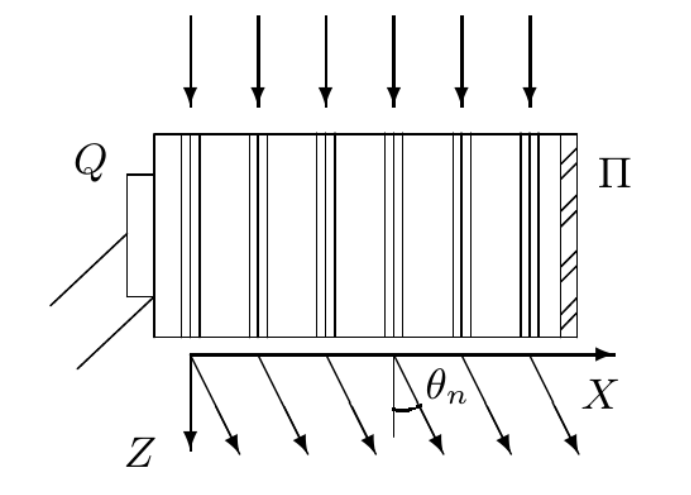
\includegraphics[width=0.5\linewidth]{img1.png}
\caption{Дифракция световых волн на акустической решетке}
\label{img1}
\end{figure}

Пусть фаза световых колебаний на передней поверхнрости жидкости равна 0. Тогда на задней она равна 
\begin{equation}
\varphi = knL = \varphi_0(1+m\cos{\Omega x})
\end{equation}
где $L$ - толщина слоя жидкости в кювете, $k$ - волновое число для света ($k=2\pi/\lambda$), $\lambda$ - длина световой волны, $\varphi_0 = kn_0L$. Таким образом, в плоскости $z=0$ фаза свтовых колебаний является периодической функцией координаты $x$, т.е. УЗ-волна в жидкости задает дифракционную решетку.

Сформулируем качественный критерий, при котором можно считать акустическую решетку чисто фазовой, т.е. рассматривать ее как тонкий фазовый экран: 
\begin{equation}
m \ll \frac{\Lambda}{L}\sqrt{\frac{\lambda}{L}}
\end{equation}
Получается, чисто фазовая акустическая решетка реализуется лишь на достаточно слабой УЗ-волне. 

В общем случае после прохождения через кювету световое поле представляет совокупность большого числа плоских волн, распространяющихся под углами, определяемыми условием:
\begin{equation}
    \Lambda\sin{\theta_m} = m\lambda \quad (m=0,\pm1,\pm2,..)
\label{4}
\end{equation}
Каждая из этих волн соответствует одному из максимумов в дифракционной решетке Фраунгофера.

Вычислить скорость $v$ распространения ультразвуковых волн в жидкости можно по формуле:
\begin{equation}
    v=\Lambda \nu
\end{equation}

\section{Экспериментальная установка}
Для наблюдения дифракции света на УЗ-волнах на оптической скамье собирается установка, изображенная на рис.\ref{img2}.

Источник света $\text{Л}$ через светофильтр $\text{Ф}$ и конденсор $K$ освещает щель $S$, которая расположена в фокусе объектива $O_1$. Выходящий из объектива параллельный пучок света прохожит через кювету $C$ перпендикулярно направлению распространения УЗ-волн. Эти волны возбуждаются в жидкости пьезоокварцевой пластинкой $Q$, прикрепленной к стенке кюветы. На кварцевую пластинку подается напряжение ультразвуковой частоты от генератора. В фокальной плоскости второго объектива $O_2$ образуется дифракционная картина, наблюдаемая при помощи микроскопа $M$.

\begin{figure}[h]
\centering
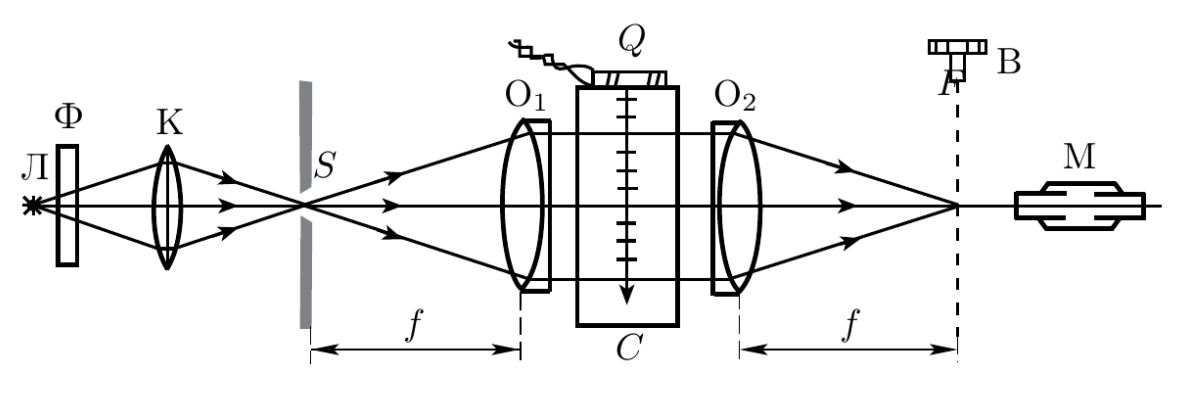
\includegraphics[width=0.8\linewidth]{img2.png}
\caption{Схема наблюдения дифракции на акустической решетке}
\label{img2}
\end{figure}

Четкость дифракционных полос зависит от ряда факторов(например, от ширины щели $S$, от ее наклона по отношению к вертикали, от угла наклона кюветы к падающему лучу).

Длина $\Lambda$ ультразвуковой волны определяется с помощью \ref{4}; в силу малости углов $\theta_m$ окончательное выражение:
\begin{equation}
    l_m=mf\frac{\lambda}{\Lambda}
\end{equation}
где $l_m$ - измеренное на опыте линейное расстояние между $m$-м и нулевым максимумами, а $f$ - фокусное расстояние объектива $O_2$.

\section{Наблюдение оптических неоднородностей, создаваемых ультразвуковыми волнами в жидкости, методом темного поля}
Для получения видимого изображения фазовой акустической решетки необходимо получить в поле зрения микроскопа изображение задней плоскости кюветы. Это достигаеся с помощью вспомогательной положительной линзы $O$, которую располагают на оптической скамье за фокальной плоскостью объектива $O_2$(рис. \ref{img3})

\begin{figure}[h]
\centering
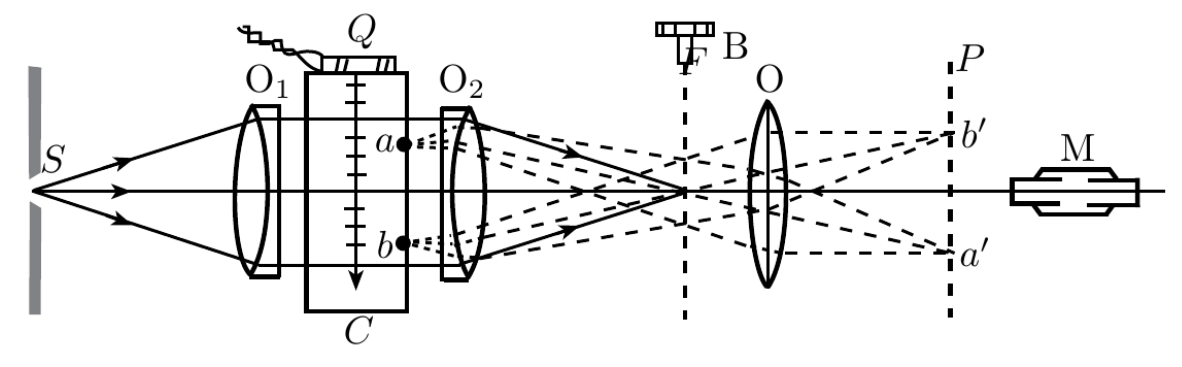
\includegraphics[width=0.8\linewidth]{img3.png}
\caption{Наблюдение акустической решетки методом темного поля}
\label{img3}
\end{figure}

Перемещая микроскоп вдоль оптической скамьи, фокусируют его на плоскость $P$, где расположено четное изображение $a'b'$ предмета $ab$, вплотную прижатого к стенке кюветы.

Для наблюдения пространственной структуры фазовой решетки можно использовать методы \textit{фазового контраста} или \textit{темного поля}. Фазовую структуру можно сделать видимой при изменении фазы колебаний в центральном дифракционном максимуме на $\pm\pi/2$. Такой метод наблюдения наз. \textit{метод фазового контраста}. В этой работе используется \textit{метод темного поля}, основанный на устранении центрального дифракционного максимума с помощью специального экрана. В поле зрения микроскопа будут наблюдаться чередующиеся светлые и темные полосы, причем расстояние между темными полосами соотвествует смещению в плоскости кюветы на $\Lambda/2$. Должно наблюдаться характерное для этого метода удвоение числа деталей рассматриваемой структуры.

\section{Установка с горизонатальной щелью}
Источник света $\text{Л}$(рис.\ref{img4}) с помощью конденсора $K$ проецируется на входную (коллиматорную) щель $S$. Входная щель ориентирована горизонтально и прикрыта красным светофильтром $\text{Ф}$. Коллиматорный объектив $O_1$ посылает параллельный пучок на кювету с водой $C$.

Излучатель $Q$, погруженный в кювету, создает УЗ-волну. Вертикальное перемещение излучаетля осуществляется винтом I(рис.\ref{img5})

\begin{figure}[h]
\centering
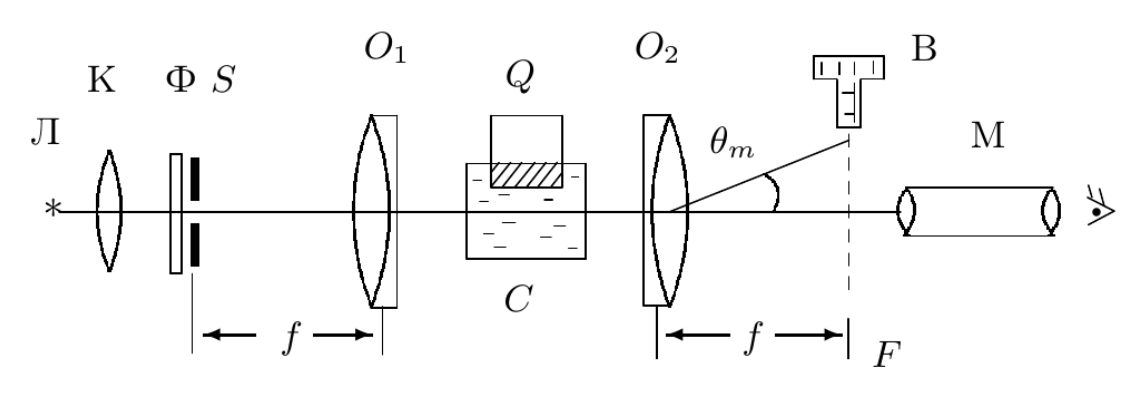
\includegraphics[width=0.8\linewidth]{img4.png}
\caption{Схема для наблюдении дифракции на акустической решетке}
\label{img4}
\end{figure}

\begin{figure}[h]
\centering
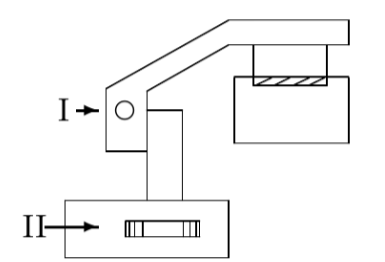
\includegraphics[width=0.3\linewidth]{img5.png}
\caption{Устройство для вертикального перемещения излучателя}
\label{img5}
\end{figure}

\begin{figure}[h]
\centering
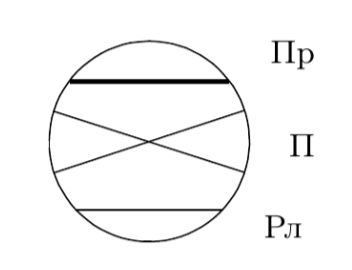
\includegraphics[width=0.3\linewidth]{img6.png}
\caption{Проволока $\text{П}_P$ перекрестие П и реперная линия $P_\text{Л}$ в фокальной плоскости объектива $O_2$}
\label{img6}
\end{figure}

Параллельный пучок света, дифрагируя на стоячей звуковой волне, образует дифракционную картину в фокальной плоскости $F$ (рис.\ref{img4}) камерного объектива $O_2$. Картинку можно наблюдать в микроскоп $M$.

Дифракционные полосы ориентированы горизонтально. Расстояние между инми можно измерить с помощью микрометрического винта $B$. Винт передвигает размещенные на стекле (рис.\ref{img6}) в плоскости $F$ перекрестие $\text{П}$, тонкую реперную линию $P_\text{Л}$ и толстую проволоку $\text{П}_P$, которая используется в методе темного поля.

\section{Ход работы}
\subsection{I. Определение скорости ультразвука по дифракционной картине}

\begin{enumerate}
    \item Собираем схему согласно рис.\ref{img4}. Включаем осветитель. Максимально открываем входную щель.
    
    Настраиваем приборы и устанавливаем рабочую ширину щели 20-30 мкм. 
    \item Получаем в поле зрения микроскопа дифракционную картину

    Перемещая излучатель с помощью лимба, оценим по порядку величины длину УЗ-волны как удвоенное расстояние между наиболее четкими дифракционными картинами.

    Определим рабочую частоту: $\nu = 1.0900\text{МГц}$

    Оценим скорость звука в воде: $v=\Lambda\nu=$
    \item Определим положения дифракционных полос:
    \begin{enumerate}
        \item меняя частоту генератора, найдем дифракционную картину
        \item вращением лимба добиваемся наилучшей картины
        \item с помощью перекрестия и микрометрического винта определим координату $Y$ каждой светлой полосы:
    \end{enumerate}
    \item Повторим измерения для нескольких частот
    
    \begin{table}[h!]
    \centering
    \begin{tabular}{||c|c|c||c|c|c||c|c|c||}
        \multicolumn{3}{ c }{$\nu = 1.09169\text{Мгц}$} & \multicolumn{3}{ c }{$\nu = 1.03036\text{МГц}$} & \multicolumn{3}{ c }{$\nu = 1.06489\text{МГц}$} \\
        \hline
        m & y, дел & y, мкм & m & y, дел & y, мкм & m & y, дел & y, мкм\\
        \hline
        -2 & 63 & 252 & -2 & 60 & 240 & -2 & 64 & 256 \\
        -1 & 24 & 196 & -1 & 24 & 196 & -1 & 25 & 100 \\
        0 & 0 & 0 & 0 & 0 & 0 & 0 & 0 & 0 \\
        1 & 33 & 132 & 1 & 29 & 116 & 1 & 30 & 120 \\
        2 & 60 & 240 & 2 & 58 & 232 & 2 & 60 & 240 \\
        \hline
    \end{tabular}
    \end{table}

    \begin{table}[h!]
    \centering
    \begin{tabular}{||c|c|c||c|c|c||}
    \multicolumn{3}{ c }{$\nu = 1.15895\text{МГц}$} & \multicolumn{3}{ c }{$\nu=1.12559\text{МГц}$} \\
        \hline
        m & y, дел & y, мкм & m & y,дел & y, мкм \\
        \hline
        -2 & 70 & 280 & -2 & 61 & 244 \\
        -1 & 27 & 108 & -1 & 24 & 96 \\
        0 & 0 & 0 & 0 & 0 & 0 \\
        1 & 34 & 136 & 1 & 34 & 136 \\
        2 & 64 & 256 & 2 & 66 & 264 \\
        \hline
    \end{tabular}
    \end{table}

    \item Для подготовки установки к следующему упражнению, глядя в окуляр, закроем проволочкой центральный максимум. 
    \item Построим графики $Y=Y(m)$ (от $-m$ до $+m$). 
    \newpage
    \begin{figure}[h]
    \centering
    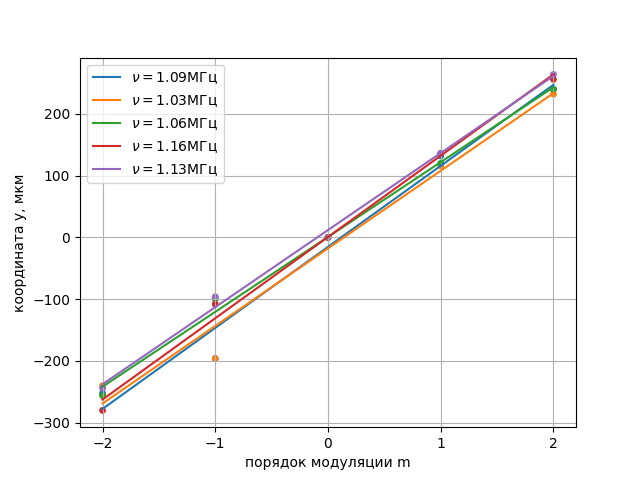
\includegraphics[width=0.8\linewidth]{graph1.png}
    \caption{Зависимость координаты $y$ от порядка модуляции $m$}
    \label{graph1}
    \end{figure}
    
    Для каждой частоты определим по наклону прямой расстояние между соседними полосами. Зная фокусное расстояние объектива $O_2$ ($f$=28см) и полосу пропускания красного фильтра ($\lambda=6400\pm200A$), рассчитаем длину УЗ-волны $\Lambda$, и скорость звука для каждой частоты, и среднюю скорость.
    
    \begin{table}[h!]
    \centering
    \begin{tabular}{||c|c|c|c||}
    \hline
        $\nu$, МГц & $l_m$, мкм & $\Lambda$, мм & $v$, м/с \\
        \hline
        1.09 & 131.2 & 1.366 & 1491.1 \\ 
        1.03 & 125.6 & 1.427 & 1470.1 \\
        1.06 & 121.2 & 1.478 & 1574.5 \\
        1.16 & 131.6 & 1.362 & 1578.1 \\
        1.13 & 124.8 & 1.436 & 1616.2 \\
        \hline
    \end{tabular}
    \end{table}

    Средняя скорость: $\overline{v}$ = (1546.00$\pm$4.45) м/c

    \subsection{II. Определение скорости ультразвука методом темного поля}

    \item Для перехода к методу темного поля отодвигаем микроскоп от щели и размещаем в промежутке между ними дополнительную линзу.

    Поднимаем излучатель над кюветой, опускаем в воду квадратную сетку и прижимаем ее к задней по ходу луча стенке кюветы.

    Настраиваем видимость сетки и рассчитываем цену малого деления окулярной шкалы в этом эксперименте:  $30 \cdot 0.02 = 0.6$ мкм.
    \item Для наблюдения акустической решетки устанваливаем рабочую ширину щели. Убираем калибровочную сетку из кюветы, опускаем туда излучатель и, варьируя частоту, постараемся увидеть звуковую решетку в микроскоп. 
    \item Закрываем нулевой дифракционный максимум проволокой.
    \item Меняя частоту, наблюдаем акустическую решетку.
    \item Перемещая излучатель, найдем наиболее четкую картину звуковой решетки. Определим с помощью окулярной шкалы микроскопа координаты первой и последней из хорошо видимых в поле зрения темных полос и количество светлых промежутков между ними.
    \item Повторяем измерения для других частот:

    \begin{table}[h!]
    \centering
    \begin{tabular}{||c|c|c|c|c|c||}
    \hline
        $\nu$, МГц & y1, дел & y1, мкм & y2, дел & y2, мкм & N \\
        \hline\hline
        2.04457 & 0.14 & 0.084 & 3.3 & 1,980 & 20 \\
        1.71041 & 0.22 & 0.132 & 3.26 & 1.956 & 17 \\
        1.50219 & 0.14 & 0.084 & 3.18 & 1.908 & 15 \\
        1.82202 & 0.08 & 0.048 & 3.28 & 1.968 & 17 \\
        2.08881 & 0.06 & 0.036 & 3.30 & 1.980 & 20 \\
        1.37896 & 0.32 & 0.192 & 3.18 & 1.908 & 13 \\
        \hline
    \end{tabular}
    \end{table}

    \item Для каждой частоты рассчитаем длину УЗ-волны $\Lambda$ с учетом удвоения числа наблюдаемых полос
    \begin{table}[h!]
    \centering
    \begin{tabular}{||c||c|c|c|c|c|c||}
    \hline
        $\nu$, МГц & 2.04457 & 1.71041 & 1.50219 & 1.82202 & 2.08881 & 1.37896 \\
         \hline
        $\Lambda$, мм & 0.945 & 0.835 & 0.737 & 0.922 & 0.679 & 0.793 \\
        \hline
    \end{tabular}
    \end{table}

    \item Построим график $\Lambda=F(\frac{1}{\nu})$ и определим по наклону прямой скорость ультразвука в воде.

    \begin{figure}[h]
    \centering
    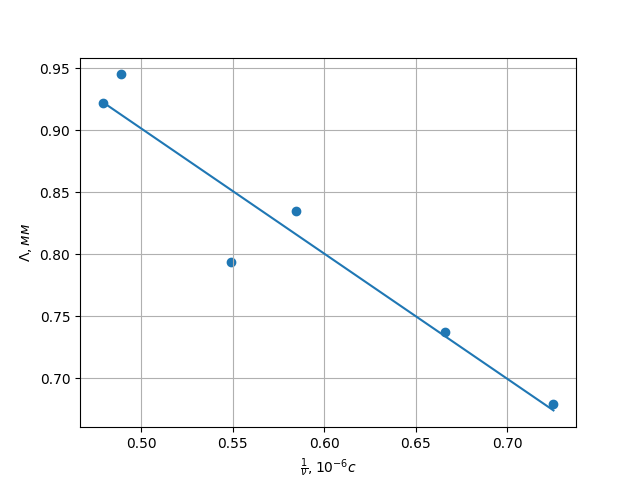
\includegraphics[width=0.8\linewidth]{graph2.png}
    \caption{Зависимость длины волны $\Lambda$ от $\frac{1}{\nu}$}
    \label{graph2}
    \end{figure}

    Коэффициент наклона прямой(скорость звука в воде): $v=(1462.44\pm5.61)$м/c

    \item Сравним значения:
    $$
    v_\text{дифкар} = (1546.0\pm4.5) \text{м/c}
    $$
    $$
    v_\text{темпол} = (1462.4\pm5.6)\text{м/c}
    $$
\end{enumerate}

\section{Выводы}
Мы изучили дифракцию света на синусоидальной акустической решетке и пронаблюдали фазовую решетку методом темного поля. Мы рассчитали скорость звука в воде двумя способами. Полученные значения близки к табличному.
\end{document}
